\section{Architecture and Code Review}
\label{sec:architecture_review}
In this section, we review the architecture of the three services of the Basilisk platform.
We point out possible problems with the previous implementations and list missing implementations that need to be added.


\subsection{Code Refactoring}
\label{sec:code_refactor}
Code refactoring is the process of restructuring the source code of an application without changing its functionality \cite{fowlerRefactoringImprovingDesign2019a}.
Some inconsistencies in the code style and duplicate code snippets have been found during the code analysis.
In other parts, the code structure differed from the design patterns recommended for the Spring and Spring Boot framework.

In general, in-depth code refactoring was recommended to increase the readability and maintainability of the source code. 


\subsection{Management of Repositories and Configurations}
\label{sec:management_repo_config}
Previously, the observed repositories were managed and stored in the \ac{hcs} while the configurations for the \tsp{} were managed and stored in the \ac{jms}.
This made it difficult to internally link a repository to a \ts{} configuration since they were stored in different services.

The previous implementations tried to solve this problem by sending events about repository creations from the \ac{hcs} to the \ac{jms}.
This resulted in the duplication of the repository storage in both services.
This contradicted the idea of microservice, which should be separated as much as possible from each other.

Therefore we recommended restructuring the management of repositories.


\subsection{Creation and Management of Benchmarking Jobs}
\label{sec:creation_of_benchmark_jobs}
When a new release is found by the \ac{hcs}, the \acl{jms} will create and manage benchmarking jobs which will be executed by the \ac{tbs}.
Previously, the \ac{jms} had created multiple jobs.
For each query file, a job was created for each dataset.
This means that each dataset was mixed with each query file, which led to queries executed on the wrong datasets.

A benchmark should only use a defined pair of a matching query file and dataset.
Therefore, the logic for creating the benchmark jobs had to be changed, and the data model for storing the benchmark jobs.


\subsection{Data Model Restructure}
\label{sec:review_data_model}
The \ac{jms} manages and stores the different configuration types needed for a benchmark job.

The configurations are stored in an internal database.
Figure \ref{fig:jms_db_schema} shows the previous database schema.

The schema had logical errors and was, in parts, incomplete.
In the following, we list some inconsistencies and possible problems that we noticed:
\begin{itemize}
	\item The only way to identify a repository as \gh{} or \dockh{} repository was to check in the \ts{} configuration.
		If a repository was assigned to the wrong type, the resulting benchmark job was not executable because \gh{} and \dockh{} need to be handled differently during a benchmark, as explained in section \ref{sec:ts_benchmarking_service}.
	
	\item Each \ts{} configuration could have exactly one \gh{} or \dockh{} repository.
		This means that for every repository, a new \ts{} configuration had to be added.
		There are fewer duplicate configurations if multiple repositories point to the same configuration.
		For example, a hook is set up to observe a \gh{} repository for new releases, and another hook is set up to observe the same \gh{} repo for pull requests.
		In this case, both hooks are using the same \ts{} configuration since it is the same \ts{} that gets benchmarked.
		
	\item As explained in section \ref{sec:creation_of_benchmark_jobs}, the creation and storage of benchmark jobs had to be changed.
		Previously, the data model structure for benchmark jobs, datasets, and query files were too complicated.
		Since the creation process of the jobs had to be changed, the data model was also changed, and the model relationships were cleaned up.
	
\end{itemize} 

Therefore, the data model for the \ac{jms} had to be restructured to cover real world requirements better.

\begin{figure}[tbph]
	\centering
	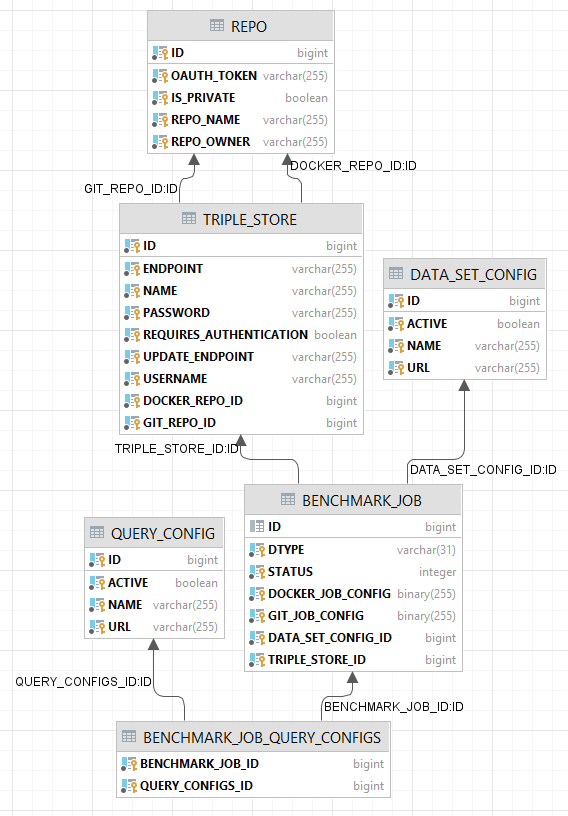
\includegraphics[width=.7\textwidth]{figures/jms_db_schema.png}
	\caption{Diagram of the previous database schema used in the \ac{jms}}
	\label{fig:jms_db_schema}
\end{figure}



\subsection{Missing Implementations}
\label{sec:review_missing_impl}
The Basilisk platform was not yet fully implemented.
After reviewing the source code, the following overview was created.

\subsubsection{\acl{hcs}}
The implementation of the \acl{hcs} was well developed.
Small additions had to be implemented.

\begin{itemize}
	\item The REST endpoints for deleting \gh{} and \dockh{} repositories had to be added.
	
	\item Previously Pull Requests for \gh{} repositories could not be observed.
\end{itemize}


\subsubsection{\acl{jms}}
The implementation of the \acl{jms} was mainly missing the REST API and some internal logic.
The following REST endpoints had to be added:

\begin{itemize}
	\item Adding / removing \ts{} configurations
	
	\item Adding / removing benchmark configurations
		\begin{itemize}
			\item Adding / removing dataset configurations
			
			\item Adding / removing query configurations
		\end{itemize}
\end{itemize}

Since the \ac{jms} also manages the running and pending benchmark jobs, the REST API and internal logic for managing these jobs had to be implemented too.

\begin{itemize}
	\item List running / pending jobs and their status
	
	\item Aborting a benchmark job
\end{itemize}



\subsubsection{\acl{tbs}}
The implementation of the \acl{tbs} previously contained only a few classes for the data models and simple structures of service classes.
Significant parts of the logic had still to be implemented.

Existing classes were mainly for storing and manipulating data models, configurations, and basic message queue interactions.
These classes did not carry much functionality.

The main functionality of the \ac{tbs} had to be implemented.
This consisted of setting up the Docker containers which contain the \tsp{} for benchmarking:

\begin{itemize}
	\item Pulling Code from \gh{}
	\item Pulling images form \dockh{}
	
	\item Building Docker containers from Dockerfiles / Docker Images
	
	\item Connecting to the Docker containers
\end{itemize}

Further, the usage of the \iguana{} framework had to be implemented.
The framework had to be set up to write the benchmark results to the \acl{jsts}.
\\

To have better control of the running jobs and the benchmarking service in general, we recommended adding a small REST API to the \ac{tbs}.
This API is similar to the one of the \ac{hcs}, which starts and stops the continuous checking.
The API for the \ac{tbs} functions like a switch, which indicates if a new benchmarking job will be started or not.
If it is set to off, the current benchmarking job will be finished, but no new job will be started.

Lastly, after performing a benchmark, the cleanup of the Docker containers had to be implemented.

\subsection{User Management and Security}
\label{sec:review_user_management}
The Basilisk platform has no user management and access control implemented.
Currently, the REST APIs of the services allow interactions with any user.
If the platform is needed to run publicly, some user management and further security measures are needed.
That includes registering new users and user groups with different user rights.
Some users should only be able to read benchmark results, while other users should be able to create repositories and abort jobs.

Secondly, confidential information needs to be kept secret.
This is, for example, the OAuth-Key needed for accessing private \gh{} repositories.


\newpage
\subsection{Frontend}
\label{sec:review_frontend}
The frontend introduces new programming languages and frameworks.
A short review of the current source code resulted in the following findings:
\begin{itemize}
	\item Currently, only a small web view is implemented
	\item Functionality to communicate with the REST APIs is missing
\end{itemize}


As explained in section \ref{sec:time_schedule}, the priority for the frontend has been lowered.
The priority of the thesis lies in finishing the main services and their functionality.

